% Pacotes e configurações padrão do estilo ``article''\
% -------------------------------------
\documentclass[a4paper,11pt]{article}
% Layout
% ------------------------------------------------------------------------------
%     Gráficos e layout ----------------------------------------------------------------------

\ifx\pdfmatch\undefined
\else
    \usepackage[T1]{fontenc}
    \usepackage[utf8]{inputenc}
\fi
% xetex:
\ifx\XeTeXinterchartoks\undefined
\else
    \usepackage{fontspec}
    \defaultfontfeatures{Ligatures=TeX}
\fi
% luatex:
\ifx\directlua\undefined
\else
    \usepackage{fontspec}
\fi
% End engine-specific settings

%      Fonte --------------------------------------------------------------------------------
%\usepackage{lmodern}
\usepackage{times}
%     Pacotes adicionados -------------------------------------------------------------------
\usepackage{ae}
%     Língua e hifenização ------------------------------------------------------------------
\usepackage[portuguese]{babel}
\usepackage{hyphenat}
%      Outros --------------------------------------------------------------------------------
\usepackage{hyperref} % Permite Links personalisados usando hyperref
\usepackage{fancyhdr}
\usepackage{sectsty}
\usepackage{float}   % Gerencia melhor o posicionamento das figuras e tabelas
%\usepackage{graphicx}
\usepackage[pdftex]{color,graphicx}
\usepackage{hyperref}
\usepackage{enumerate} % Permite alterar Layout do enumerate
%\usepackage{pdflscape}  % Permite alterar a orientação da pagina para Paisagem
%\usepackage{ifthen}  % Permite usar condicionais ifelse
%\usepackage[table]{xcolor} % Permite alterar as cores das células de uma tabela
\usepackage{amsmath,amssymb} % Ambiente para uso de elementos matemáticos
\usepackage{caption}
\usepackage{subcaption} % permite o uso de multiplas figuras com legenda (ambiente subfigure)
%\usepackage{minted} % Ambiente minted para colorir código de programas
\usepackage{natbib} % Para referencia bibliográfica
\usepackage{url}    % Referência de links na internet
%\usepackage{listings} % pacote para apresentar código de programação
\usepackage{indentfirst}  % Para indentar o primeiro parágrafo de cada seção
\usepackage{titling}  % Permite Montar uma página de titulo própria

% Layout do documento ------------------------------------------------------------------------
%     Bordas e tamanho da página ------------------------------------------------------------
\usepackage{geometry} 
 \geometry{ % Padrõa ABNT para relatórios
 a4paper,
 left=30mm,
 right=20mm,
 top=30mm,
 bottom=20mm
 }
%     Cabeçalho e Rodapé ---------------------------------------------------------------
\pagestyle{fancy}
  \lhead{}
  \chead{}
  \rhead{}
  \lfoot{}
  \cfoot{}
  \rfoot{\thepage}
%     Númeração ------------------------------------------------------------------------
  \pagenumbering{arabic}
%     Retas do cabeçalho e rodapé ------------------------------------------------------
  \renewcommand{\headrulewidth}{0.5pt}
  \renewcommand{\footrulewidth}{0.5pt}
%     Tamanho da letra de seções e derivadas --------------------------------------------
  \sectionfont{\normalsize}
  \subsectionfont{\small}
%     Hiperlinks ------------------------------------------------------------------------
  \hypersetup{
                  colorlinks,
                  citecolor=black,
                  filecolor=black,
                  linkcolor=black,
                  urlcolor=black
                  }
%     Definições do pdf ----------------------------------------------------------------------
\hypersetup{
    unicode=false,          % non-Latin characters in Acrobat’s bookmarks
    pdftoolbar=true,        % show Acrobat’s toolbar?
    pdfmenubar=true,        % show Acrobat’s menu?
    pdffitwindow=false,     % window fit to page when opened
    pdfstartview={FitH},    % fits the width of the page to the window    
    pdfauthor={Rafael Lima},     % author
    pdfnewwindow=true      % links in new window
}
%     Outros ----------------------------------------------------------------------------
      %\renewcommand{\thesection}{(\alph{section})} % muda o estilo de númeração das sections
      % alterando a formatação dos numeradores de lista de itens
      \renewcommand\theenumi{\arabic{enumi}}
      \renewcommand\labelenumi{(\textit{\theenumi})}
	  \renewcommand\theenumii{\arabic{enumii}}
	  \renewcommand\labelenumii{(\textit{\theenumi.\theenumii})}
      
% ---------------------------------------------------------------------------------------


\usepackage{circuitikz}
\usepackage[makestderr]{pythontex}

\title{Laboratório 1} % Define o título do Relatório
\author{Rafael Lima}

% Definições Auxiliares ( Macros próprias )
% ------------------------------------------------------------------------------
%\input{relat_aux.tex} % Arquivo com minhas macros
\newcommand{\npy}[1]{\sympy{round(#1,4)}}
% ----------------------------------~>ø<~---------------------------------------
\begin{document}
% Capa e Índice ----------------------------------------------------------------
%--------------------------------------------------- Capa --------------------------------------------
%\newpage
\begin{figure}[h!]
\centering

\includegraphics[scale=0.9]{img/simb_unb.png}
\label{fig:unb}
\end{figure}

\begin{center}
{\LARGE Universidade de Brasília}\\
Departamento de Engenharia Elétrica\\
Professor: Henrique Cezar Ferreira\\
Disciplina: Controle Digital\\
\end{center}


\vspace{0.18\textheight}

\begin{center}
    \Huge \textbf{\\\thetitle \\}
\end{center}

\vspace*{\fill} % Completa espaço em branco e empurra o resto para o final da página

% Tabela com os nome das pessoas do grupo

\begin{table}[H]
    \begin{tabular}{ll}
        % Nome      & Matrícula
        Rafael Lima & 10/0131093 \\
    \end{tabular}
\end{table}

\vspace{0.5cm}

\begin{center}
    \textbf{Brasília\\
    \the\year} % Coloca o Ano atual
\end{center}

\thispagestyle{empty} % Retira o cabeçalho e o rodapé da página

% ------------------------------------------------- Índice -------------------------------------------
\newpage
\tableofcontents
\newpage
% ----------------------------------------------------------------------------------------------------

 % Capa para UnB
% Conteúdo ---------------------------------------------------------------------

\section{Análise Sistema Discreto}

% Código fonte colocado a parte para facilitar validação dentro do ipython
\begin{sympycode}
# Get Source Code
sys.path.insert(1, '../../')
from src.python.exsim1 import *
\end{sympycode}

Considerando um sistema de controle a tempo discreto com realimentação unitária e período de amostragem $T = 1s$ cuja função de transferência a malha aberta é dado pela equação \ref{eq:openloop-sys} :

\begin{equation}\label{eq:openloop-sys}
    G(z) = \sympy{nGo}
\end{equation}

Denominando $\alpha_1 = 0.3679$, $\alpha_0 = 0.2642$, $\beta_1 = 1$ temos

\begin{equation}\label{eq:openloop-sys-symbolic}
    G(z) = \sympy{sGo}
\end{equation}

Temos que a função de transferência em malha fechada do sistema é

$$G_{mf}(z) = \frac{G(z)}{G(z) + 1}$$

\begin{equation}\label{eq:closedloop-sys-symbolic}
    G_{mf}(z) = \sympy{sGc}
\end{equation}

A partir de \ref{eq:closedloop-sys-symbolic} temos que o polinômio característico de malha fechada é

\begin{equation}\label{eq:poly-sys-symbolic}
    \phi(z) = \sympy{poly}
\end{equation}

Substituindo $\sympy{a1} = \sympy{na1}$, $\sympy{a0} = \sympy{na0}$, $\sympy{b1} = \sympy{nb1}$ temos, respectivamente para o a função de transferência de malha fechada e o polinônio caractarístico as equações \ref{eq:closedloop-sys} e \ref{eq:poly-sys}.

\begin{equation}\label{eq:closedloop-sys}
    G_{mf}(z) = \sympy{nGc}
\end{equation}

\begin{equation}\label{eq:poly-sys}
    \phi(z) = \sympy{npoly}
\end{equation}

\section{Estabilidade pelo Critério de Juri}

\subsection{Definição Critério de Jury}

Para um sistema de ordem 2 as condições para estabilidade pelo critério de juri, é necessário avaliar 2+1=3 condições para verificar a estabilidade, sendo estas as seguintes:

\begin{equation}\label{eq:jury-c1}
    \phi(1) > 0
\end{equation}

\begin{equation}\label{eq:jury-c2}
    (-1)^n\phi(-1) > 0\ ,\ n=2
\end{equation}

\begin{equation}\label{eq:jury-c3}
    |A_0| < |A_n|
\end{equation}

\subsection{Avaliando primeira condição}

Calculando $\phi(1)$:

$$\phi(z) = \sympy{poly}$$
$$\phi(1) = \sympy{eqJ1}$$
$$\phi(1) = \sympy{neqJ1}$$

Se $\phi(1) > 0$ então

$$\sympy{neqJ1} > 0$$

Isolando $K$:

\begin{equation}\label{eq:k-jury-c1}
    K > \sympy{K1}
\end{equation}

Substituindo $\sympy{a1} = \sympy{na1}$, $\sympy{a0} = \sympy{na0}$, $\sympy{b1} = \sympy{nb1}$ temos

$$K > \sympy{sK1}$$

Logo a primeira condição é

\begin{equation}\label{eq:k-jury-c1-numeric}
    K > \npy{nK1.simplify()}
\end{equation}

\subsection{Avaliando segunda condição}

Dado a equação característica $\phi(z) = \sympy{poly}$ temos

$$(-1)^2\phi(-1) = \phi(-1) = \sympy{eqJ2}$$

Logo

$$\sympy{eqJ2.factor(K)} > 0$$

Isolando $K$

\begin{equation}\label{eq:k-jury-c2}
    K > \sympy{K2}
\end{equation}

Substituindo $\sympy{a1} = \sympy{na1}$, $\sympy{a0} = \sympy{na0}$, $\sympy{b1} = \sympy{nb1}$ temos

$$K < \sympy{sK2}$$

\begin{equation}\label{eq:k-jury-c2-numeric}
    K < \npy{nK2}
\end{equation}

\subsection{Avaliação terceira condição}

$$\phi(z) = \sympy{poly.expand().factor(z)}$$

$$
\left\{\begin{array}{l}
A_0 = \sympy{apoly[0]} = \sympy{napoly[0]}\\
A_1 = \sympy{apoly[1]} = \sympy{napoly[1]}\\
A_2 = \sympy{apoly[2]} = \sympy{napoly[2]}\\
\end{array}
\right.
$$

$$|A_0| < |A_2|$$
$$|\sympy{napoly[0]}| < |\sympy{napoly[2]}|$$
$$0 < |\sympy{napoly[2]}| - |\sympy{napoly[0]}|$$

Isolando $K$

\begin{equation}\label{eq:k-jury-c3-numeric}
    K < \npy{nK3}
\end{equation}

\subsection{Estabilidade}

Comparando o resultado das inequações \ref{eq:k-jury-c1-numeric}, \ref{eq:k-jury-c2-numeric} e \ref{eq:k-jury-c3-numeric} temos que o intervalo de restrição para K é

\begin{equation}\label{eq:k-jury-result}
    K < \sympy{round(min(nK2,nK3),4)}
\end{equation}

\section{Estabilidade pelo Critério de Routh modificado}

O critério de Roth originalmente foi concebido para a avaliação de estabilidade de sistemas contínuos. No entanto podemos adaptar o sistema em tempo discreto a adotando a seguinte substituição de variável

\begin{equation}\label{eq:bilinear-transf-w}
    w = \frac{z+1}{z-1}
\end{equation}

Isolando $z$ temos:

\begin{equation}\label{eq:bilinear-transf-z}
    z = \frac{w+1}{w-1}
\end{equation}

O que representar uma propriedade interessante da transformada bilinear. Substituindo \ref{eq:bilinear-transf-z} em

$$G(w) = \sympy{sGw}$$
$$G(w) = \sympy{sGw.simplify()}$$

Substituindo $\sympy{a1} = \sympy{na1}$, $\sympy{a0} = \sympy{na0}$, $\sympy{b1} = \sympy{nb1}$ temos
$$G(w) = \sympy{nGww}$$

A partir do qual temos a seguinte equação característica no $plano-w$:

\begin{equation}
    \phi_w(w) = \sympy{npolyw}
\end{equation}

% TODO Gerar tabela de Roth
% Em particular para um polinomio de grau dois basta olhar somente ultimo termo

A partir da tabela de Roth obtemos a seguinte expressão $0 < \sympy{sK4}$. Isolando $K$:

\begin{equation}\label{eq:k-roth-numeric}
    K < \npy{nK4}
\end{equation}

Comparando a expressão da inequação \ref{eq:k-roth-numeric} e \ref{eq:k-jury-result}, observa-se que foi obtido um valor similar para ambos métodos.

\section{Resposta do Sistema}

\subsection{Região de Oscilação Constante}

Com base no resultado do critério de estabilidade de Juri, se definimos $K = \sympy{K3}= \npy{nK3}$. Substituindo $K$ na função de transferência temos:

\begin{equation}\label{eq:closedloop-sys-oscilation}
    G_{2}(z) = \sympy{nGc.subs(K,nK4).simplify()}
\end{equation}

Que possui os polos 
$$p_0 = \sympy{opoles[0]}$$
$$p_1 = \sympy{opoles[1]}$$.

Desta forma podemos obter a frequência de oscilação do sistema como $f = \frac{w}{2\pi}$ em que $w = ||p_0|| = ||p_1||$.

$$f = \frac{||p_0||}{2\pi} = \frac{\npy{sympy.arg(opoles[1])}\ rad/s}{2\pi} = \npy{freq} Hz$$

Na figura \ref{fig:ex1-plot-oscilation} temos a resposta ao degrau junto de uma senoide com frequência $f = \npy{freq} Hz$. Note a resposta segue a aproximadamente a mesma forma da senoide em diversos pontos.

\begin{figure}[H]
    \label{fig:ex1-plot-oscilation}
    \centering
    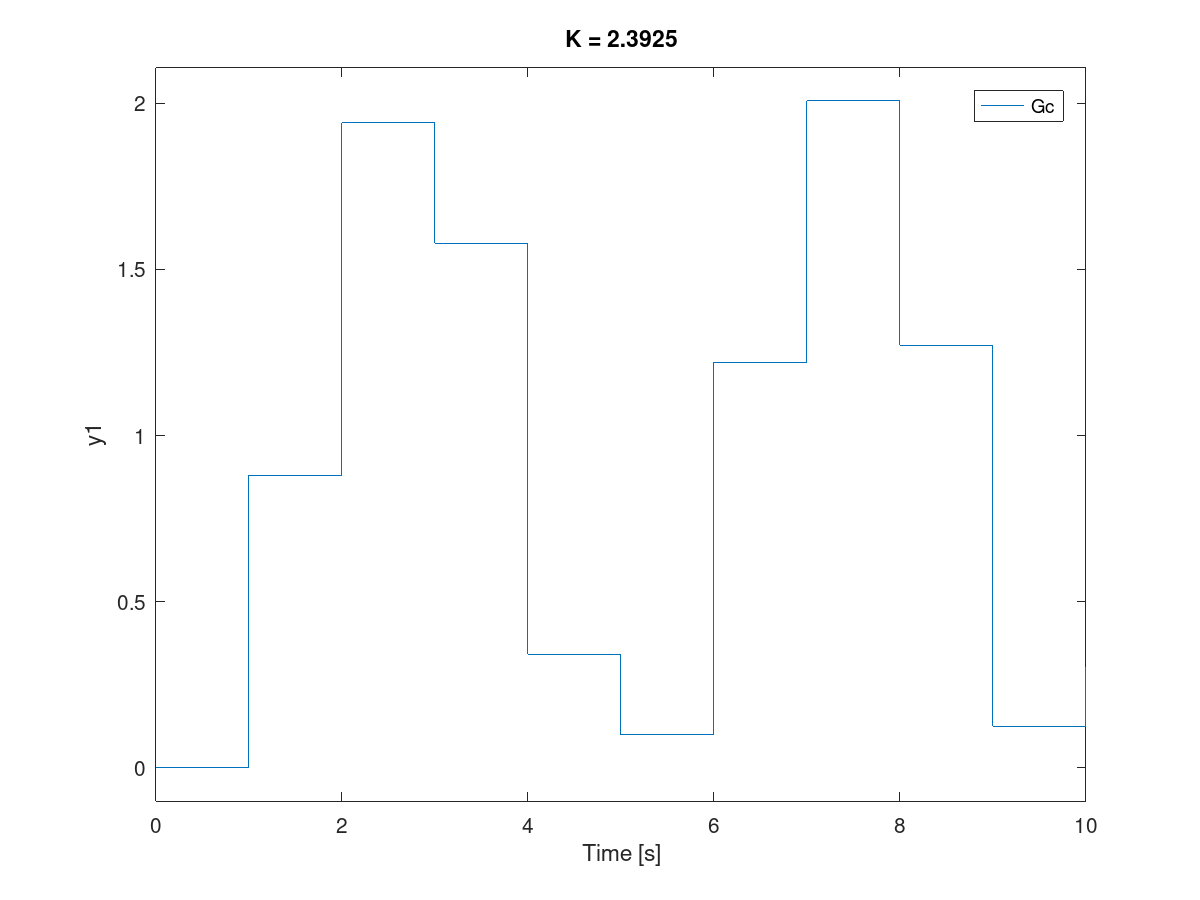
\includegraphics[width=0.9\linewidth]{img/exsim1-plot-oscilation.png}
    \caption{Resposta ao Degrau Unitário do Sistema com $K = \npy{nK3}$}
\end{figure}

\subsection{Sistema Estável}

De forma similar, pelo critério de Juri temos que, para todo valor de $0< K < \npy{nK3}$ o sistema é estável. Em particular para $K = \npy{0.5*nK3}$ temos a seguinte resposta

\begin{figure}[H]
    \centering
    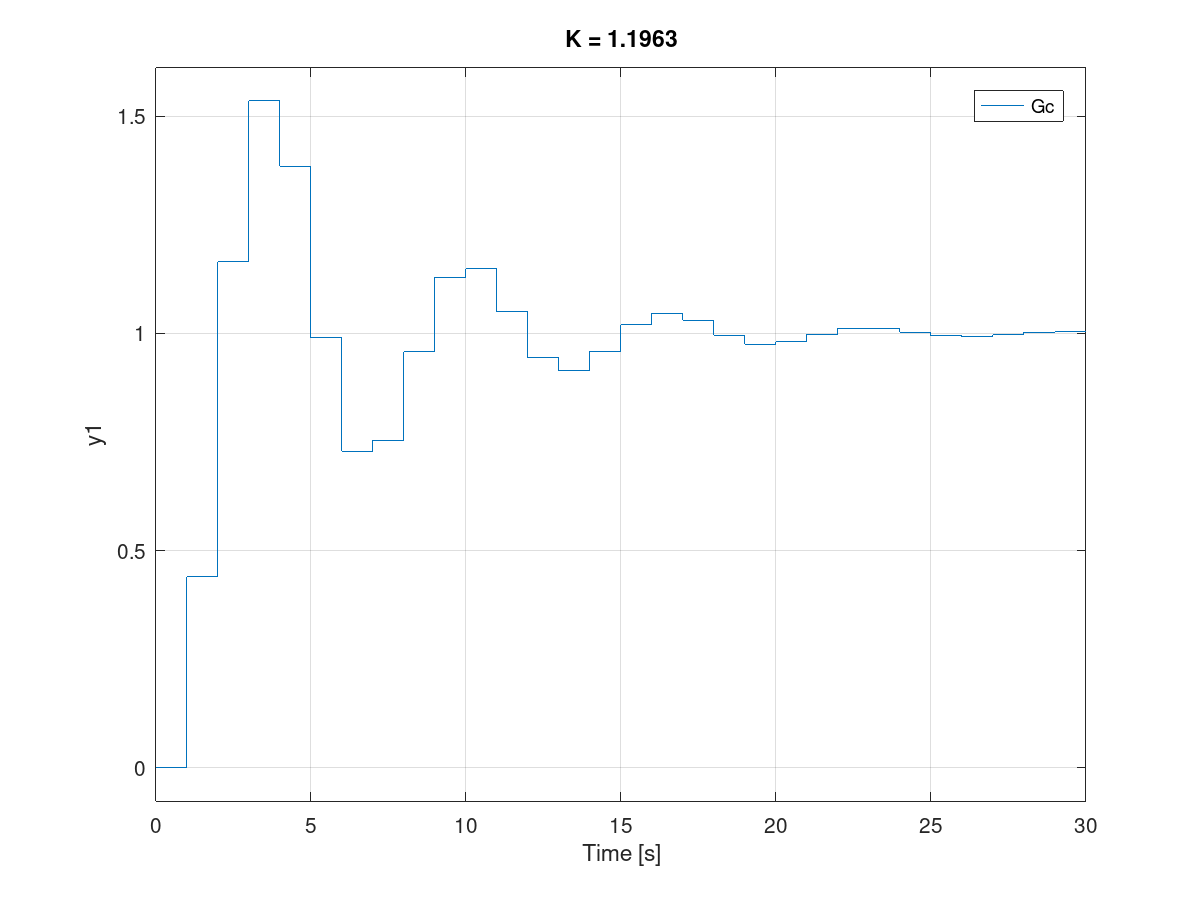
\includegraphics[width=0.9\linewidth]{img/exsim1-plot-stable.png}
    \caption{Resposta ao Degrau Unitário do Sistema com $K = \npy{0.5*nK3}$}
\end{figure}

\subsection{Sistema Instável}

Por fim, para todo valor de $K > \npy{nK3}$ o sistema é instável. Em particular para $K = \npy{2*nK3}$ temos

\begin{figure}[H]
    \centering
    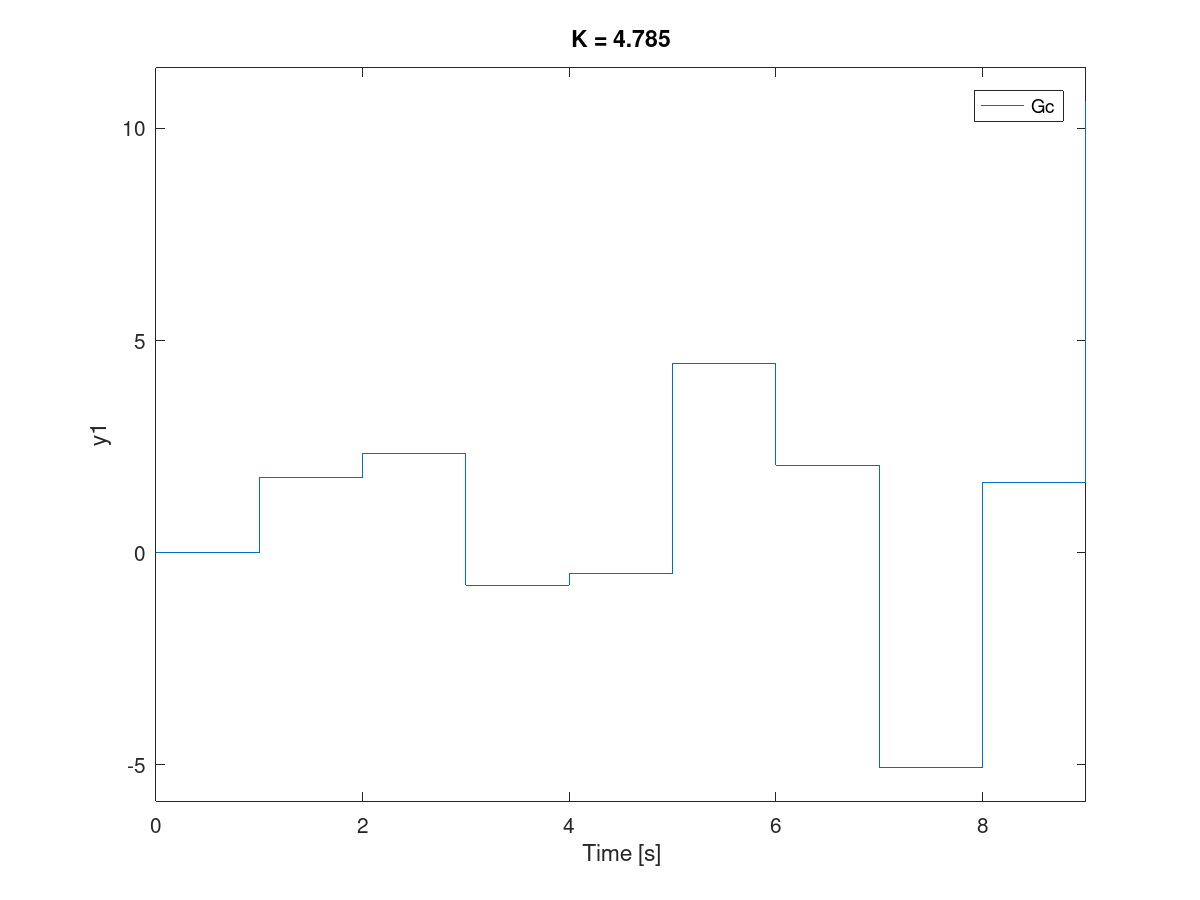
\includegraphics[width=0.9\linewidth]{img/exsim1-plot-instable.png}
    \caption{Resposta ao Degrau Unitário do Sistema com $K = \npy{2*nK3}$}
\end{figure}


\section{Conclusão}



% ------------------------------------------------------------------------------

\nocite{sympy}
\bibliographystyle{abbrv}
\bibliography{references}
% Referências
% Acrescentadas no arquivo references.bib
% para usa-las no texto batsa usar \citep{}

% ------------------------------------------------------------------------------
\section{Anexos}
\subsection{Python}

Para o avaliação da estabilidade usando o critério de Jury e o critério de Roth modificado foi utilizado o seguinte código em python:

\inputminted[xleftmargin=15pt,linenos,frame=single,framesep=5pt]{python}{../python/exsim1.py}

\subsection{Octave}

Para o desenho dos gráficos e simulações foi utlizado o \textit{octave} em conjunto do pacote \textit{control}. Segue o código referente para as simulações

\inputminted[xleftmargin=15pt,linenos,frame=single,framesep=5pt]{matlab}{../matlab/exsim1.m}


% ------------------------------------------------------------------------------
\end{document}
